\documentclass{article}
\usepackage{graphicx}
\usepackage{float}
\usepackage{gensymb}
\parskip=12pt

\begin{document}

\title{Laboratory 6: Diffraction and Interference}
\date{December 12, 2014}
\author{Calvin Chan\\304144970\\Physics 4BL Lab 8\\Partners: Caleb Choi, Stanley
Chan}

\maketitle

\section{Introduction}

This lab explores light interference and demonstrates the duality of light as,
both, a wave and a particle. It attempts to prove the validity of several
equations that govern electromagnetic waves. By measuring the interference
patterns of light through various medium (single slit, double slits, diffraction
grating, and hair), we can show how these electromagnetic waves constructively
and destructively interfere with each other.

\section{Experimental Results}

\begin{figure}[H]
    \centering
    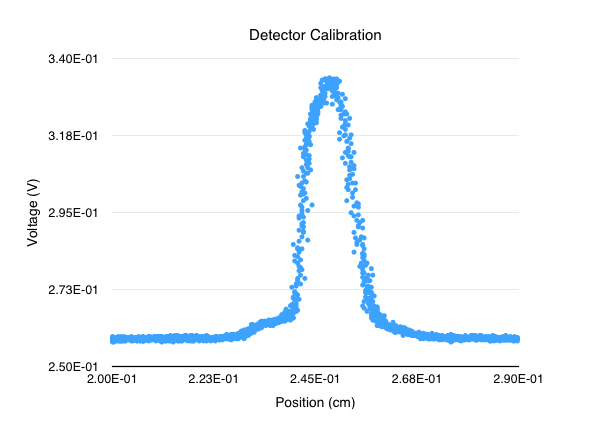
\includegraphics[width=\textwidth]{charts/calibration}
    \caption{Using a linear translator for the position/voltage conversion}
    \label{calibration}
\end{figure}

\begin{figure}[H]
    \centering
    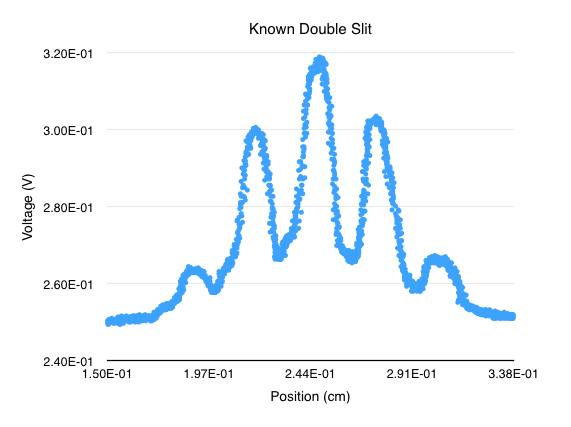
\includegraphics[width=\textwidth]{charts/known}
    \caption{Using a linear translator for the position/voltage conversion}
    \label{known}
\end{figure}

\begin{figure}[H]
    \centering
    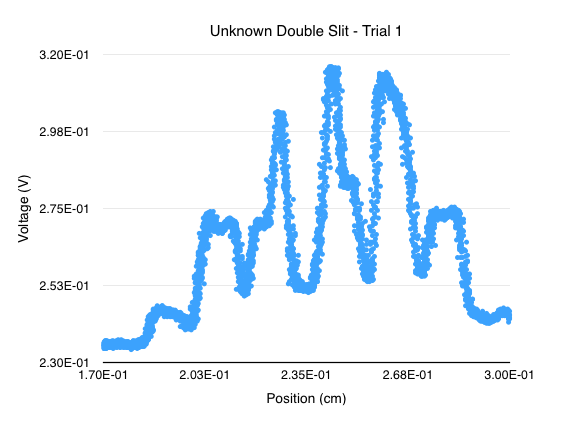
\includegraphics[width=\textwidth]{charts/unknown1}
    \caption{Using a linear translator for the position/voltage conversion}
    \label{unknown1}
\end{figure}

\begin{figure}[H]
    \centering
    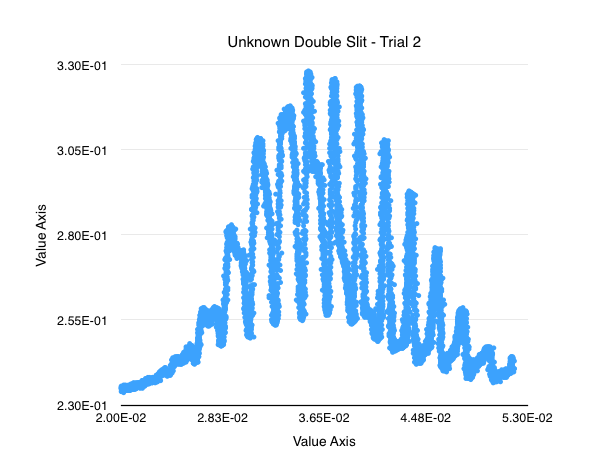
\includegraphics[width=\textwidth]{charts/unknown2}
    \caption{Using a linear translator for the position/voltage conversion}
    \label{unknown2}
\end{figure}

\begin{figure}[H]
    \centering
    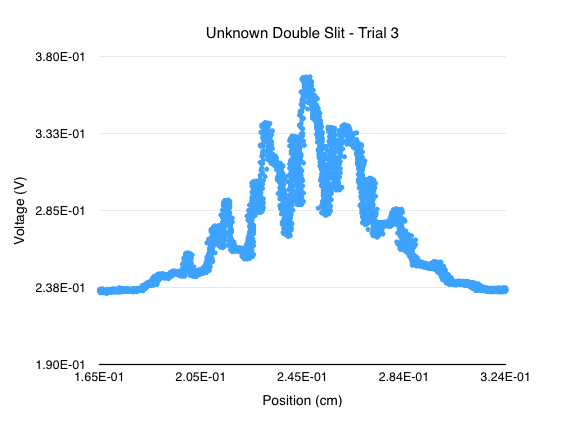
\includegraphics[width=\textwidth]{charts/unknown3}
    \caption{Using a linear translator for the position/voltage conversion}
    \label{unknown3}
\end{figure}

\section{Analysis}

\section{Conclusion}
This experiment successfully properties of thin and thick lenses, as well as
verified several equations and laws that govern such optics. Snell's Law was
successfully verified through our experiments. We were able to demonstrate the
focal length of two separate lenses in combination, as well as verify
magnification properties of images and objects. Most of our theoretical values
all fell under the acceptable value range after taking into account error
propogation and uncertainty. For the values that fell out of the range yielded
by error propogation, we can attribute the error to lack of precision in
measurements (measuring light beams with the human eye) as well as small
uncertainties in the measurement of distances. 
\end{document}
